% Author: Till Tantau
% Source: The PGF/TikZ manual
% https://texample.net/tikz/examples/all/?page=2
\documentclass{minimal}

\usepackage{tikz}
%\usetikzlibrary{trees,snakes}
\usepackage{verbatim}

\begin{document}
\pagestyle{empty}

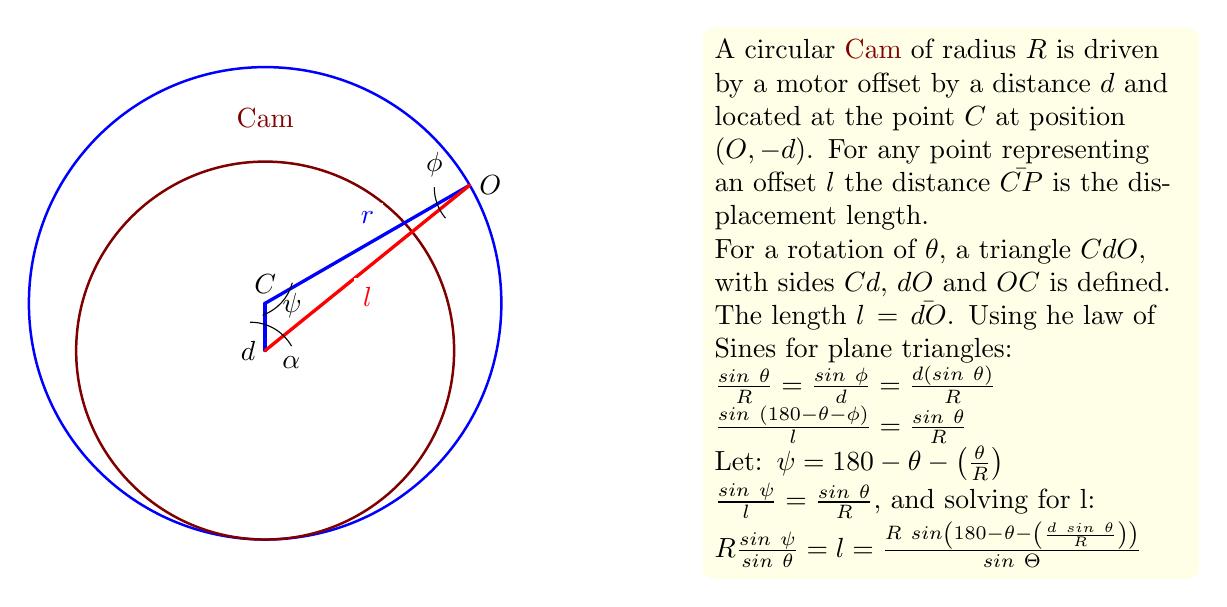
\begin{tikzpicture}[scale=3,cap=round]
  % Local definitions
  \def\costhirty{0.8660256}
  \def\camoffset{-.2}

  % Key Colors
  \colorlet{camcolor}    {red!50!black}
  \colorlet{anglecolor}  {green!50!black}
  \colorlet{sincolor}    {red}
  \colorlet{tancolor}    {orange!80!black}
  \colorlet{coscolor}    {blue}


  % Key Points
  \def\ptO{$O$}
  \def\ptC{$C$}
  \def\ptd{$d$}

  \coordinate[label=above : \ptC]  (C)     at (0,          0);
  \coordinate[label=left  : \ptd]  (d)     at (0,          \camoffset);
  \coordinate[label=right : \ptO]  (O)     at (\costhirty, .5);

  % Styles
  \tikzstyle{axes}=[]
  \tikzstyle{important line}=[very thick]
  \tikzstyle{information text}=[rounded corners,fill=yellow!10!white,inner sep=1ex]

  % The grid
  %\draw[style=help lines,step=0.5cm] (-1.4,-1.4) grid (1.4,1.4);

  \draw[color=blue,line width=0.9pt]         (0,0)   circle (1cm);
  \draw[color=red!50!black,line width=0.9pt] (0,-.2) circle (.8cm) ;
  \draw[color=red!50!black]                  (0,.7)  node[above=.1] {Cam} ;

  \draw[style=important line,coscolor] (0,0)   --  (d);
  \draw[style=important line,coscolor] (0,0)   -- node[above=3.5pt,fill=white] {$r$} (O);
  \draw[style=important line,sincolor] (0,-.2) -- node[below=3pt,fill=white]   {$l$} (O);

  % Arcs

  \draw (.1111, -.18)  node[below=.2] {$\alpha$} arc[start angle = 30,end angle = 90, radius=.2] ;
  \draw (\costhirty-.15, .49)  node[above=.2] {$\phi$} arc[start angle = 180,end angle = 220, radius=.2] ;
  \draw (-.01, -.05)   arc[start angle = 290,end angle = 345, radius=.2] node[below=.1] {$\psi$} ;

  \draw[xshift=1.85cm] node [right,text width=6cm,style=information text]
  {
    A circular {\color{camcolor} Cam} of radius $R$ is driven
    by a motor offset by a distance $d$ and located at the point $C$
    at position $(O,-d)$. For any point representing an offset $l$ the
    distance  $\bar{CP}$ is the displacement length.

    For a rotation of $\theta$, a triangle $CdO$, with sides $Cd$, $dO$ and $OC$ 
    is defined. The length $l = \bar{dO}$. Using he law of Sines for plane triangles:

   $\frac{sin~\theta}{R} = \frac{sin~\phi}{d} = \frac{d(sin~\theta)}{R}$ \\
   $\frac{sin~(180-\theta-\phi)}{l} = \frac{sin~\theta}{R}$

   Let: $\psi = 180-\theta-\left( \frac{\theta}{R} \right)$

   $\frac{sin~\psi}{l} = \frac{sin~\theta}{R}$, and solving for l:

   $R\frac{sin~\psi}{sin~\theta} = l = \frac{R~sin\left( 180 - \theta - \left( \frac{d~sin~\theta}{R} \right) \right)}{sin~\Theta}$
    };

\end{tikzpicture}

\end{document}


https://tex.stackexchange.com/questions/407751/make-a-border-around-a-circled-image

shading -- make a spectrum!
https://www.math.uni-leipzig.de/~hellmund/LaTeX/pgf-tut.pdf
